\documentclass[12pt,letterpaper]{article}
\usepackage{anysize}
\usepackage{amsmath}
\marginsize{2cm}{2cm}{1cm}{1cm}
\usepackage{listings}
\usepackage{cite}
\usepackage{caption}
\usepackage{upquote}
\usepackage{xcolor}
\usepackage{xcolor}

\usepackage{tikz}
\def\checkmark{\tikz\fill[scale=0.4](0,.35) -- (.25,0) -- (1,.7) -- (.25,.15) -- cycle;} 

\usepackage{graphicx}


\begin{document}

\begin{titlepage}
    \vspace*{4cm}
    \begin{flushleft}
    {\huge
        CS519 Project 6\\[.5cm]
    }
    {\large
        Image Manipulation in a "Magic Lens"
    }
    \end{flushleft}
    \vfill
    \rule{5in}{.5mm}\\
    Li Li

\end{titlepage}
\section{source files}
There are only three files lab5.frag, lab5.glib and lab5.vert.
\section{a simple explanation}
What I did are:\\
\begin{tabular}{ |l | c |}
  \hline                       
  \textbf{Feature} & \textbf{Status} \\ \hline
  Magnification & \checkmark \\ \hline
  Rotation & \checkmark \\ \hline
  Sharpening & \checkmark \\ \hline
  Extra Credit (circle lens) & \checkmark \\ \hline
\end{tabular}

\begin{itemize}
\item For the this \textbf{Magnification} I spent a lot of time on it, because I firstly try to do the lens work in vertex shader that is to build a synthetic lens. But I could't find a way to calculate new st coordinate with the new fraction vector. And than I went to the question notes and did it in fragment shader. Firstly, make sure the fragment is in rectangle and then magnify the value of st by actually divide it by \textbf{uMagFactor}. That is the inverse operation. In order to make magnify base on the centre of the lens, I have to subtract st first, than do magnification and finally add the centre st back.
See figure 1.
\item For \textbf{rotation}, this is not very hard. It works if I insert the rotation code between magnifying new st and adding centre st back.  See figure 2.
\item About \textbf{Sharpening}, it is pretty much the code from Image Manipulation notes. With irgb now is our newly mag and rotate vST and uT is now uSharpFactor.
\item Finally, for \textbf{extra credit}. This is just by checking if a certain point's st location is far than radius to centre st. I calculated the radius by \textit{$uDt^2*uDs^2$}.

\end{itemize}
\section{result}

\begin{figure}[p]
    \centering
    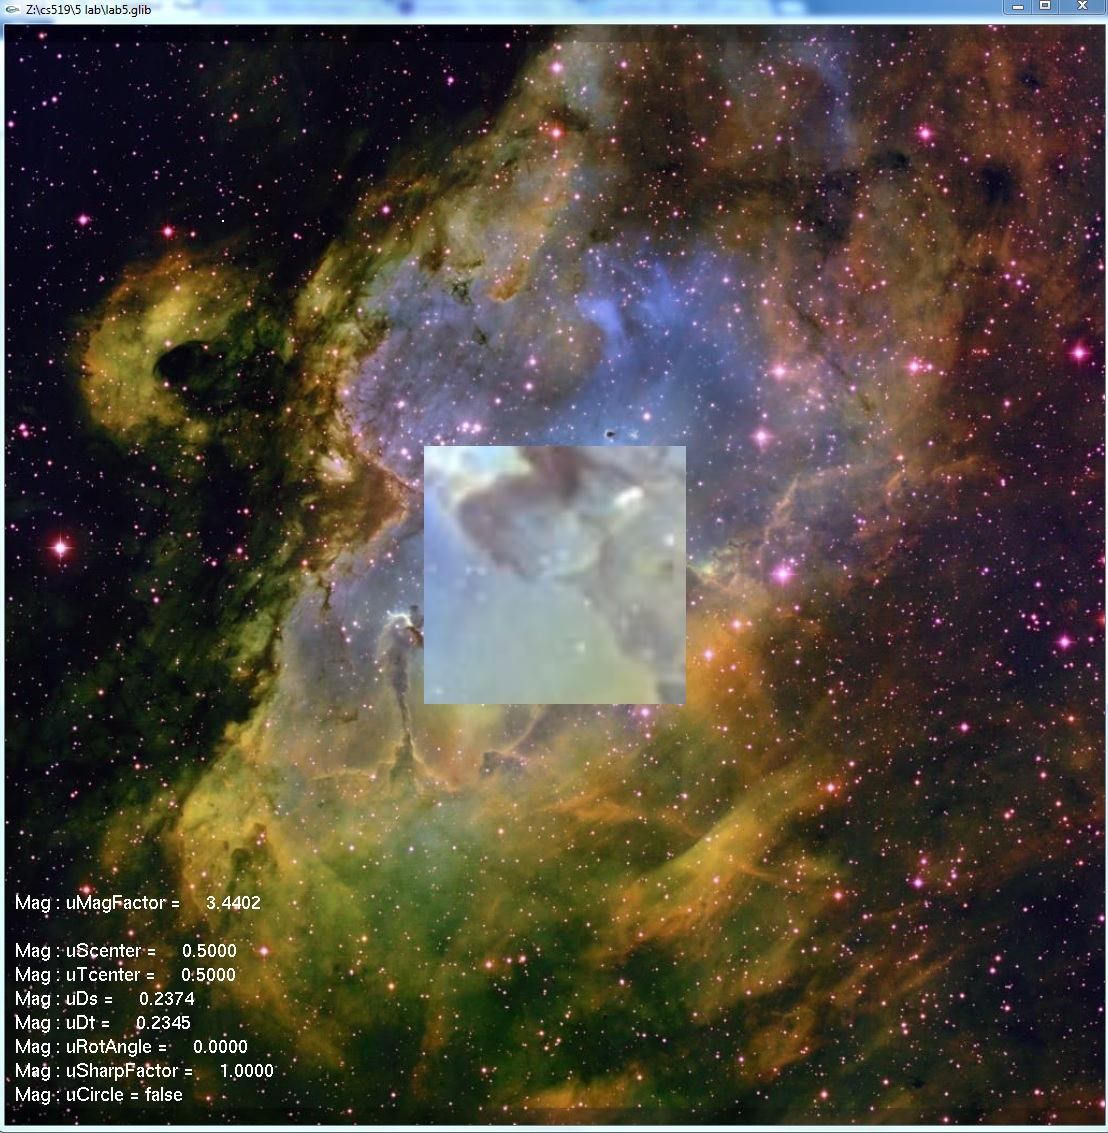
\includegraphics[width=1.0\textwidth]{1.jpg}
    \caption{Magnification}
\end{figure}

\begin{figure}[p]
    \centering
    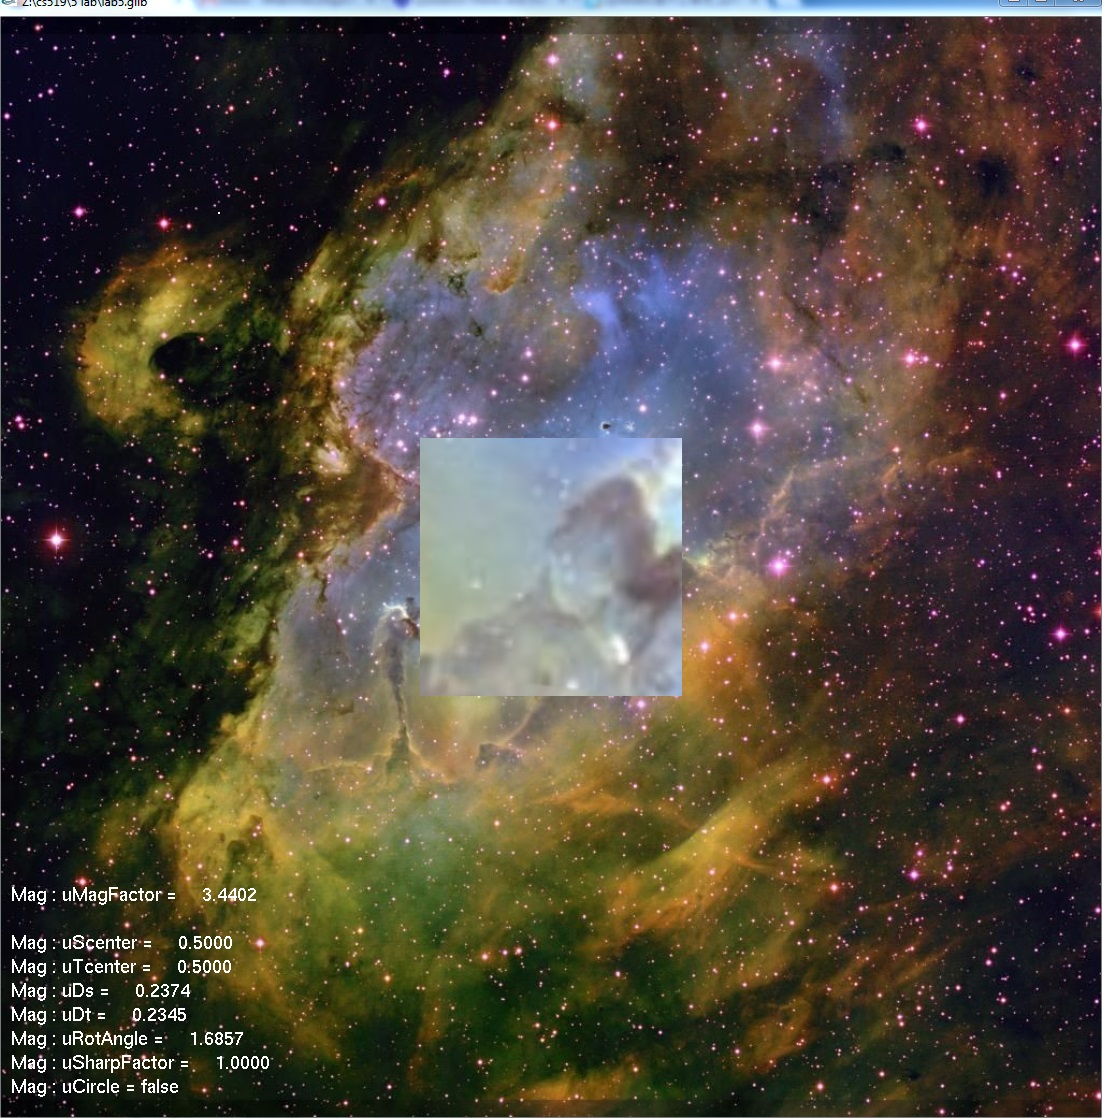
\includegraphics[width=1.0\textwidth]{2.jpg}
    \caption{Rotation}
\end{figure}

\begin{figure}[p]
    \centering
    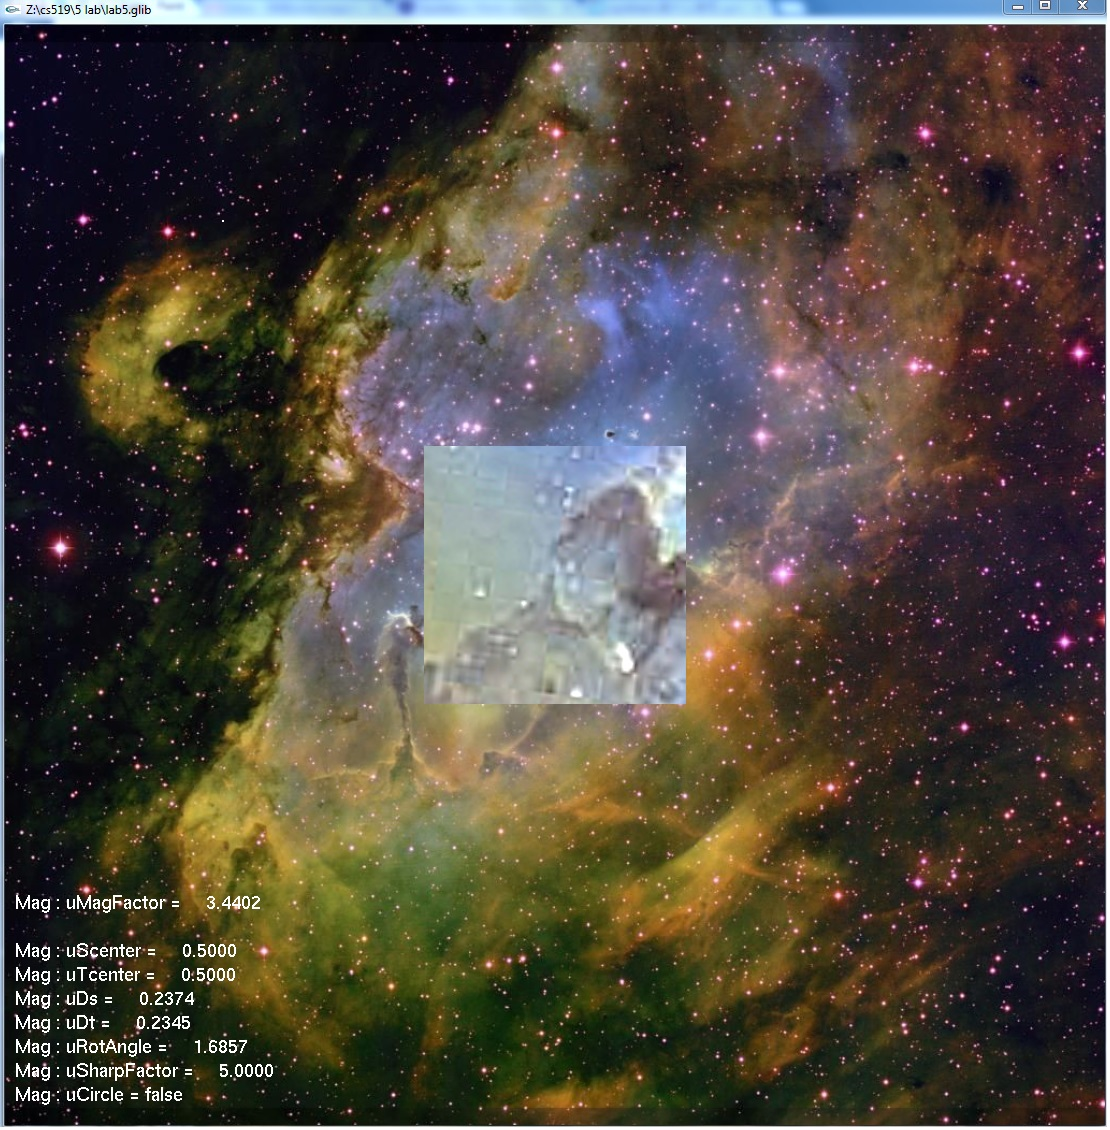
\includegraphics[width=1.0\textwidth]{3.jpg}
    \caption{Sharpening}
\end{figure}

\begin{figure}[p]
    \centering
    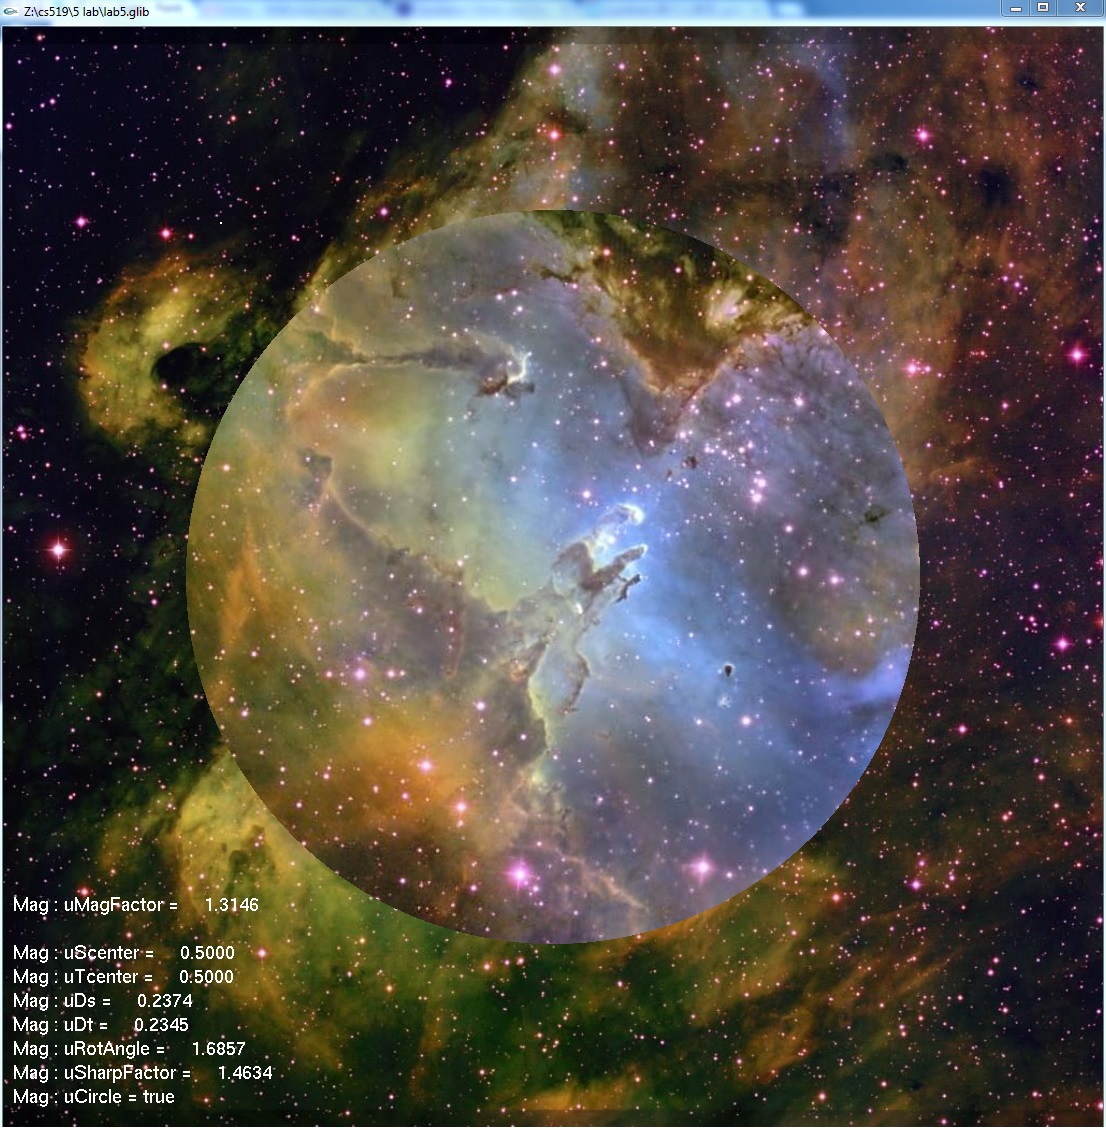
\includegraphics[width=1.0\textwidth]{4.jpg}
    \caption{Do with circle lens}
\end{figure}

\end {document}
